\documentclass{article} %% Bestimmt die allgemeine Formatierung der Abgabe.
\usepackage{a4wide} %% Papierformat: A4.
\usepackage[utf8]{inputenc} %% Datei wird im UTF-8 Format geschrieben.
%% Unter Windows werden Dateien je nach Editor nicht in diesem Format
%% gespeichert und Umlaute werden dann nicht richtig erkannt.
%% Versucht in diesem Fall "utf8" auf "latin1" (ISO 8859-1) wechseln.
\usepackage[T1]{fontenc} %% Format der Zeichen im erstellten PDF.
%\usepackage[german]{babel} %% Regeln für automatische Worttrennung.
\usepackage{fancyhdr} %% Paket um einen Header auf jeder Seite zu erstellen.
\usepackage{lastpage} %% Wird für "Seite X von Y" im Header benötigt.
                      %% Damit das funktioniert, muss pdflatex zweimal
                      %% aufgerufen werden.
\usepackage{enumerate} %% Hiermit kann der Stil der Aufzählungen
                       %% verändert werden (siehe unten).

\usepackage{amssymb} %% Definitionen für mathematische Symbole.
\usepackage{amsmath} %% Definitionen für mathematische Symbole.
\usepackage{amsthm}
\usepackage{gensymb} %% Für das Grad-Zeichen
\usepackage[export]{adjustbox} %% Für die Positionierung von Bildern
\usepackage{float}
\usepackage{caption}
\usepackage{subcaption}

\usepackage{stmaryrd}

\usepackage{tikz}  %% Paket für Grafiken (Graphen, Automaten, etc.)
\usetikzlibrary{automata} %% Tikz-Bibliothek für Automaten
\usetikzlibrary{arrows}   %% Tikz-Bibliothek für Pfeilspitzen

%% Linke Seite des Headers
\lhead{\course\\\semester\\Übungsblatt \homeworkNumber}
%% Rechte Seite des Headers
\rhead{\authorname\\Seite \thepage\ von \pageref{LastPage}}
%% Höhe des Headers
\usepackage[headheight=36pt]{geometry}
%% Seitenstil, der den Header verwendet.
\pagestyle{fancy}

\newcommand{\authorname}{Max Jappert, Maximilian Barth}
\newcommand{\semester}{Frühjahrsemester 2021}
\newcommand{\course}{Computergrafik}
\newcommand{\homeworkNumber}{4}


\usepackage[T1]{fontenc}
%\usepackage{inconsolata}

\usepackage{color}

\definecolor{dkgreen}{rgb}{0,0.6,0}
\definecolor{gray}{rgb}{0.5,0.5,0.5}
\definecolor{mauve}{rgb}{0.58,0,0.82}

\lhead{\course\\\semester\\Übungsblatt \homeworkNumber}
\rhead{\authorname\\Seite \thepage\ von \pageref{LastPage}}

\usepackage{listings}
\lstset{frame=tb,
  language=Java,
  aboveskip=3mm,
  belowskip=3mm,
  showstringspaces=false,
  columns=flexible,
  basicstyle={\small\ttfamily},
  numbers=none,
  numberstyle=\tiny\color{gray},
  keywordstyle=\color{blue},
  commentstyle=\color{dkgreen},
  stringstyle=\color{mauve},
  breaklines=true,
  breakatwhitespace=true,
  tabsize=3
}

\begin{document}
\section*{Aufgabe 8 - Theoriefragen}

Shadow Mapping funktioniert, indem der z-Buffer-Algorithmus aus Sicht der Lichtquelle ausgeführt wird, um ein Korrespondenzbild mit Tiefeninformationen (die Shadow Map) zu berechnen. Anschliessend wird beim Shading bei jedem Punkt in Weltkoordinaten nachgeschaut, ob dessen Tiefe aus Sicht der Lichtquelle grösser ist als der gespeicherte Tiefenwert an derselben Stelle in Kamerakoordinaten. Falls dem so ist, so liegt der Punkt in Weltkoordinaten im Schatten.

Die aus der Perspektive der Lichtquelle betrachteten Punkte entsprechen nicht genau den Pixel aus der Sicht der Kamera. Diese inhärente Ungenauigkeit kann Artefakte zur Folge haben, die sich in Form von Eigenbeschattung äussern. Dieses Problem kann umgangen werden, indem ein Wert (der Shadow Bias) zum Tiefenwert des Shadow Maps hinzu addiert wird.

Die folgenden Beispiele sind Produkte unserer Implementation:

\begin{figure}[H]
     \centering
     \begin{subfigure}[b]{0.4\textwidth}
         \centering
         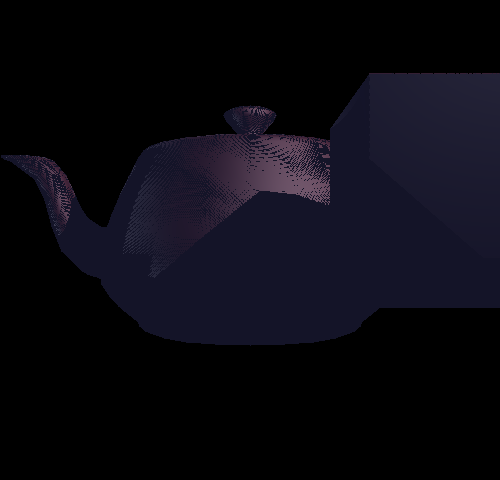
\includegraphics[width=\textwidth]{phong.png}
         \caption{Artefakte beim Phong'schen Reflektionsmodell ohne hinzuaddierten Shadow Bias.}
         \label{fig:y equals x}
     \end{subfigure}
     \hfill
     \begin{subfigure}[b]{0.4\textwidth}
         \centering
         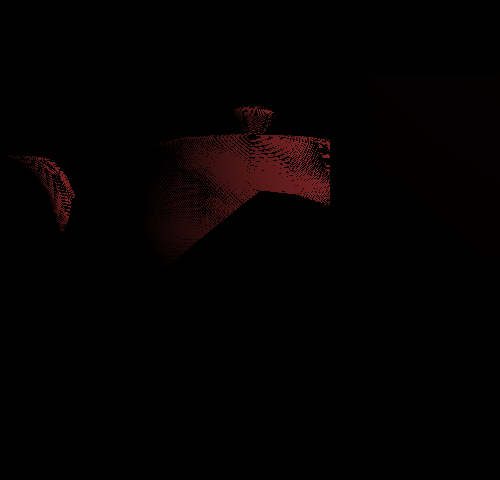
\includegraphics[width=\textwidth]{reflectance.png}
         \caption{Artefakte beim perfekten Lambert'schen Strahler ohne hinzuaddierten Shadow Bias.}
         \label{fig:three sin x}
     \end{subfigure}
\end{figure}

\end{document}